% !TEX TS-program = pdflatex
% !TEX encoding = UTF-8 Unicode

\documentclass[11pt]{article} % `twocolumn` in options

\usepackage[utf8]{inputenc} % set input encoding
\usepackage{geometry} 
  \geometry{letterpaper} 
  \geometry{margin=20mm} 
\usepackage{graphicx} % for \includegraphics 
\usepackage[parfill]{parskip} 
\usepackage{booktabs} % for much better looking tables 
\usepackage{hyperref} % https://www.overleaf.com/learn/latex/Hyperlinks
\hypersetup{
	colorlinks	= true,
	urlcolor	= NavyBlue,
	linkcolor	= NavyBlue,
	citecolor 	= ForestGreen
}
\usepackage{xspace}
\usepackage{amsmath}
\usepackage[dvipsnames]{xcolor}  % http://en.m.wikibooks.org/wiki/LaTeX/Colors
\usepackage{soul}     % for the highlight command \hl{}

\usepackage[modulo]{lineno}
\linenumbers
\modulolinenumbers[1]
\renewcommand{\linenumberfont}{\tiny\color{gray}}

%%% HEADERS & FOOTERS
\usepackage{fancyhdr} % This should be set AFTER setting up the page geometry
\pagestyle{fancy} % options: empty , plain , fancy
\renewcommand{\headrulewidth}{0pt} % customise the layout...
\lhead{}\chead{}\rhead{}
\lfoot{}\cfoot{\thepage}\rfoot{}

%%% SECTION TITLE APPEARANCE
\usepackage{sectsty}
\allsectionsfont{\sffamily\mdseries\upshape} 

%%% MACROS

\newcommand{\ie}{\textit{i.e.,}\xspace}
\newcommand{\Ro}{\ensuremath{\mathcal{R}_0}\xspace}

\newcommand{\warning}[1]{\textcolor{RedOrange}{\textbf{#1}}}


% =========================================================================
% =========================================================================

\title{\textsf{REEM - Model Description}}
\author{David Champredon}
%\date{} 

\begin{document}
\maketitle


This is the description of the REEM epidemic model. REEM stands for Renewal Equation based Epidemic Model. Unlike most implementations of epidemic models that are either based on differential equations or agent-based models, here the model is implemented with a renewal equation, with a discrete daily time step and is stochastic.

\section{Pathogen transmission}

We consider an infectious pathogen spreading in a closed population os size $N$. The number of individuals susceptible to infection on day $t$ is noted $S(t)$. 
Let $I(t)$ be the incidence on day $t$, \Ro the basic reproduction number.
The intrinsic generation interval distribution of the pathogen is noted $g$. 

The infection process is described by the following discrete-time equations:

\begin{eqnarray}
\label{eq:reinc}
j(t) & = & \Ro \left(\frac{S(t)}{N}\right)^{\exp(\alpha)} B(t) \sum_{k=1}^{t-1} g(k)\, j(t-k) \\ 
I(t) & \sim & \mathrm{Pois}(j(t))   \\
S(t) & = & \max(0, S(t-1) - I(t))
\end{eqnarray}

The time-dependent variable $j(t)$ represents the \emph{mean} incidence driven by a \emph{deterministic} pathogen transmission process.
The actual incidence at time $t$, $I(t)$, is simply drawn from a Poisson distribution with mean $j(t)$.
The parameter $\alpha$ is a real number affecting the tail-end of the epidemic curve and has been asociated with a simple way to model transmission heterogeneity. When $\alpha=0$, contacts are modelled as homogeneous (like in the canonical ODE-based SIR model). 
The deterministic function $B$ is introduced to model exogen changes in the transmission rate (for example, to represent public health interventions). When $B(t) = 1$ for all times $t$, there is no change in the intrinsic transmission rate and the epidemic follows its ``natural'' course. 

\subsection{Interpretation of the parameter $\alpha$}

The fraction $S(t)/N$ in \autoref{eq:reinc} represents the proportion of the population that is \emph{available} to be infected at time $t$. 
If contacts among individuals of the population are completely random and homogeneous, then the fraction of the population that is potentially \emph{exposed} to infection is indeed $S(t)/N$. This is because any infectious individual has a probability $S(t)/N$ to contact a susceptible individual. 

However, in reality, contacts are not truely homogeneous because of the intrinsic structures of human populations (eg, households, workplaces, social events, etc.). Hence, the actual average proportion of susceptible individuals exposed to an infectious person may either be larger (if infectious individuals ``seek'' susceptibles) or lower (if infectious individuals tend to cluster together more than with susceptibles). 
The relationship between the susceptible fraction that is exposed and the one effectively exposed can be modelled with a power law. A negative power does not really make sense in this context, so it is parameterised with an exponential, $\exp(\alpha$), to ensure its positivity.
Examples of a power-law relationship is illustrated in \autoref{fig:alpha}. 

\begin{figure}[h]
\begin{center}
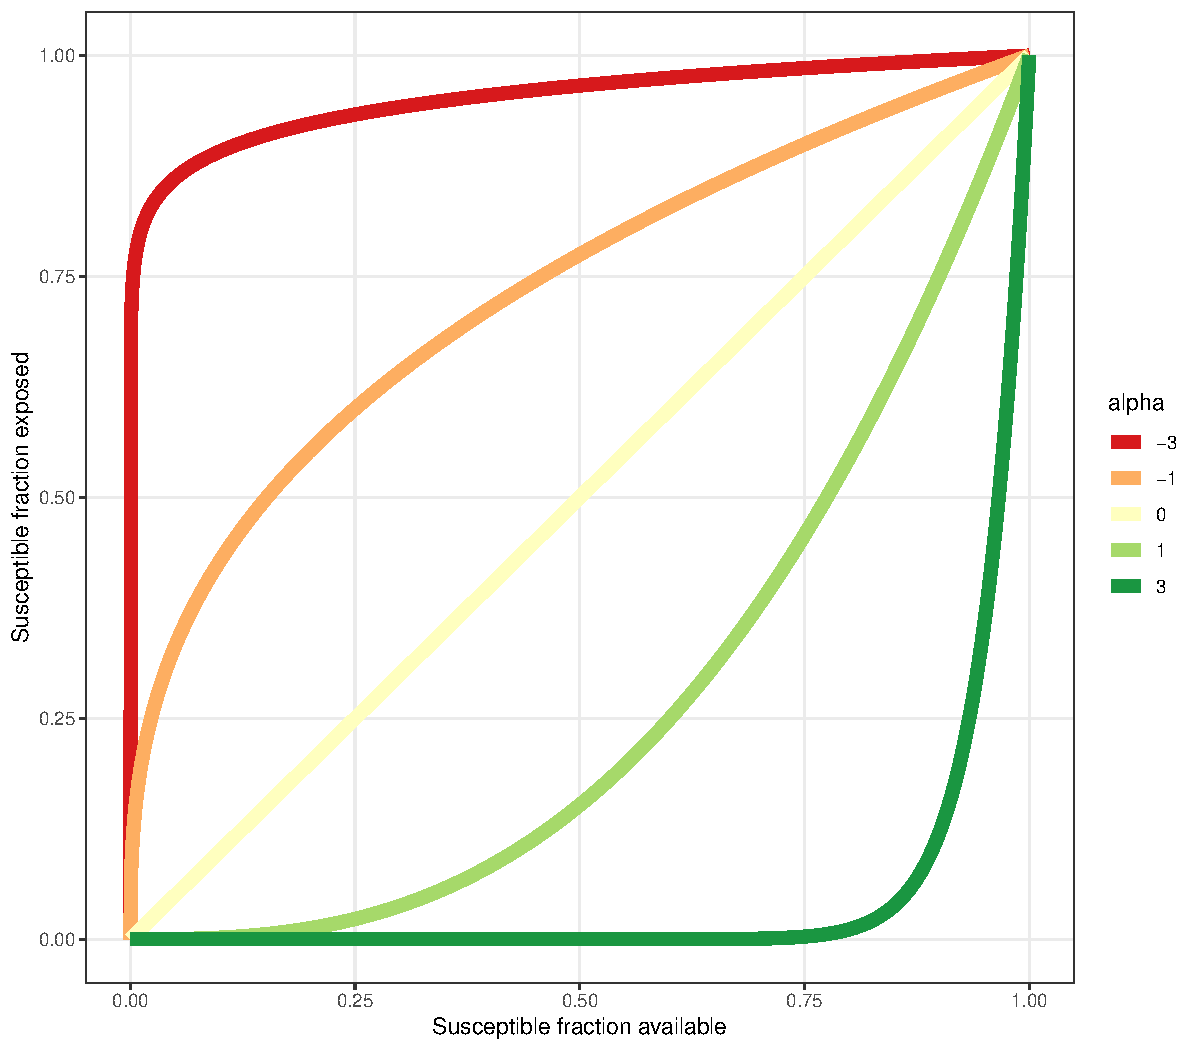
\includegraphics[width=0.5\textwidth]{alpha.pdf}
\caption{Relationship between the fraction of susceptible individuals that are effectivelly exposed to infection, as a function of the fraction of susceptible individuals that are available in the population.}
\label{fig:alpha}
\end{center}
\end{figure}

\section{Fecal/urinary shedding in wastewater}

We assume that fecal and/or urinary shedding of pathogen RNA/DNA occurs during the course of infection of an individual. In communities where a sewer system exists, a large amount of pathogen RNA/DNA is deposited in wastewater. Sampling wastewater at strategic locations (e.g., a wastewater treatment plant) and measuring the pathogen RNA/DNA concentration (using molecular techniques like qPCR or ddPCR) can indicate the prevalence of infections in the community. 
Although shedding can occur throught both fecal and urinary routes, here we simply focus on the fecal route for simplicity. 

Fecal shedding depends on pathogen. Here, we focus on a description inspired by SARS-CoV-2, as this is the most studied fecal shedding to date. 
Fecal shedding occurs shortly after infection (although we do not know exactly how long after), probably peaks around the time of symptoms onset and carries on several days after the infection has been ``cleared'' (i.e., the individual has effectively recovered, and is not diseased any more). 
 
The fecal shedding distribution, noted $f$, gives the \emph{average} amount of pathogen RNA/DNA shed with time by one infected individual. 
More precisely, $f(\tau)$ is the average amount of RNA/DNA shedded $\tau$ days after infection. 

There were $I(t-k)$ individuals infected at time $t-k$ and all have been infected for $k$ days at time $t$, hence they contribute $f(k) \times I(t-k)$ RNA/DNA copies in the wastewater on day $t$. Then, we sum over all past cohorts infected $k$ days ago. 
Hence, the amount of RNA/DNA deposited on day $t$ in wastewater by the population is:
\begin{equation}
W_d(t) = \sum_{k=1}^{t-1} f(k) \, I(t-k)
\end{equation}

Wastewater can travel long distances (several kilometers) before reaching the sampling location determined for epidemiological surveillance. The sewer system can generate complex fluid dynamics where RNA/DNA can settle and resuspend.
Hence, there can be a significant delay between the time RNA/DNA is deposited in the wastewater and the time it reaches the sampling location. 
Moreover, the wastewater is a harsh environment which can degrade RNA/DNA during its journey between the shedding and sampling points. 
We model the concentration present at the sampling site on day $t$ as:
\begin{equation}
W_p(t) = \sum_{k=1}^{t-1} \psi(k) W_d(t-k) e^{-\kappa k}
\end{equation}

The parameter $\kappa$ represents the average RNA/DNA decay in wastewater and the function $\psi$ the average time lag for the RNA/DNA copies to reach the sampling point from the shedding point.

Finally, the RNA/DNA concentration in wastewater reported depends on multiple steps performed in a laboratory. Each step generates measurement error that is simply modelled as a Gaussian process. 
The reported concentration for a sample collected at time $t$ is defined as
\begin{equation}
W_r(t) = \mathcal{N}(W_p(t), \sigma_w)
\end{equation}



\section{Hospital admissions}

Like fecal shedding in wastewater, the number of hospital admissions is modelled as simply resulting from incidence, with a time lag. 
More precisely, we define $h$ as the average fraction of infected individuals that will be hospitalized because of the severity of their infection. 
The function $h$ is the distribution of the time lags between infection and hospital admission. In other words, $h(\tau)$ is the proportion of individuals infected $\tau$ days ago that will be hospitalized today. 
Hence, the number of hospital admissions on day $t$ is given by:
\begin{equation}
H(t) = \sum_{k=1}^{t-1} h(k) \, I(t-k)
\end{equation}

%Note that a cohort of infected individuals infected at the same time in the past will contribute the fraction $\sum_{k>0} h(k)$ of its size to hospital admissions (hence, $h$ must sum less than 1).
For implementation convenience, the function $h$ is reparameterized such that the time repartition and the total quantity of hospital admissions are separated:
\begin{equation}
h(k) = \frac{\eta(k)}{\sum_{i>0}\eta(i)} \, h^\star
\end{equation}
Hence, a cohort of infected individuals infected at the same time in the past will contribute the fraction $\sum_{k>0} h(k) =  h^\star$ of its size to hospital admissions. The repartition of the hospital admission lags is defined with the unitless function $\eta$.

%\subsection{A subsection}
%
%More text and there is also \autoref{fig:example}. \warning{This is a warning}.
%
%
%\begin{figure}[h]
%\begin{center}
%\includegraphics[width=0.2\textwidth]{C:/Users/DCHAMPRE/Pictures/frog.jpg}
%\caption{Write the caption here...}
%\label{fig:example}
%\end{center}
%\end{figure}
%
%\bibliographystyle{plain}
%\bibliography{filename}

\end{document}
